%&tex

\documentclass{beamer}

\usepackage[english]{babel}
\usepackage[utf8]{inputenc}
\usepackage{mathtools}
\usepackage{amsthm}
\usepackage{amssymb}
\usepackage{thmtools,thm-restate}
\usepackage{amsfonts}
\usepackage{hyperref}
\usepackage[singlelinecheck=false]{caption}
\usepackage[backend=biber,url=true,doi=true,eprint=false,style=authoryear]{biblatex}
\usepackage{algorithm}
\usepackage[noend]{algpseudocode}
\usepackage{listings}
\usepackage{subcaption}
\usepackage{xcolor}
\usepackage{multicol}

\usepackage{graphicx}
\usepackage{tikz}
\usetikzlibrary{positioning}
\usetikzlibrary{shapes.geometric}
\usetikzlibrary{fit}
\usetikzlibrary{calc}

\usepackage{tkz-graph}

\addbibresource{references.bib}
\usetheme{Boadilla}

\DeclareMathOperator*{\argmin}{arg\,min}
\DeclareMathOperator*{\argmax}{arg\,max}
\DeclareMathOperator*{\Val}{\text{Val}}
\DeclareMathOperator*{\Ch}{\text{Ch}}
\DeclareMathOperator*{\Pa}{\text{Pa}}
\DeclareMathOperator*{\Sc}{\text{Sc}}
\newcommand{\ov}{\overline}
\newcommand{\tsup}{\textsuperscript}

\newcommand\defeq{\mathrel{\overset{\makebox[0pt]{\mbox{\normalfont\tiny\sffamily def}}}{=}}}

\newcommand{\algorithmautorefname}{Algorithm}
\algrenewcommand\algorithmicrequire{\textbf{Input}}
\algrenewcommand\algorithmicensure{\textbf{Output}}
\algnewcommand{\LineComment}[1]{\State\,\(\triangleright\) #1}

\newcommand{\Left}{\text{LEFT}}
\newcommand{\Right}{\text{RIGHT}}
\newcommand{\Up}{\text{UP}}

\newcommand{\set}[1]{\mathbf{#1}}
\newcommand{\pr}{\text{P}}
\newcommand{\eps}{\varepsilon}
\newcommand{\ddspn}[2]{\frac{\partial#1}{\partial#2}}
\newcommand{\iddspn}[2]{\partial#1/\partial#2}
\newcommand{\indep}{\perp}
\renewcommand{\implies}{\Rightarrow}

\newcommand{\bigo}{\mathcal{O}}
\newcommand{\mbf}[1]{\mathbf{#1}}

\setbeamertemplate{theorems}[ams style]

\setbeamersize{description width=1.0cm}

\lstset{frameround=fttt,
	numbers=left,
	breaklines=true,
	keywordstyle=\bfseries,
	basicstyle=\ttfamily,
}

\newcommand{\code}[1]{\lstinline[mathescape=true]{#1}}
\newcommand{\mcode}[1]{\lstinline[mathescape]!#1!}

\title[Self-driving with SPNs]{End-To-End Imitation Learning of Lane Following Policies Using
Sum-Product Networks}
\date{ENIAC 2019}
\author[R. Geh, D. Mauá]{Renato Lui Geh \and Denis Deratani Mauá}
\institute[IME-USP]{Institute of Mathematics and Statistics \\\scriptsize University of São Paulo}

\begin{document}

\maketitle

\begin{frame}
  \frametitle{Sum-product networks}

  Sum-product networks (SPNs) are deep tractable density estimators with a neural network-like
  structure subject to only sums and products as activation functions.

  \begin{center}
    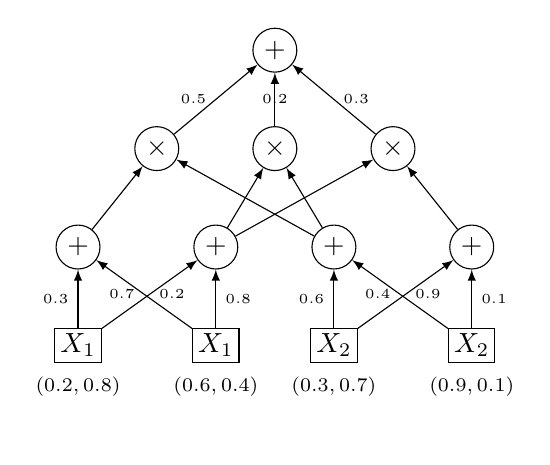
\begin{tikzpicture}
      \begin{scope}[every node/.style={circle,draw,inner sep=2pt}]
        \node (root) at (0, 0) {$+$};
        \node (p1) at (-1.5, -1.25) {$\times$};
        \node (p2) at (0, -1.25) {$\times$};
        \node (p3) at (1.5, -1.25) {$\times$};
        \node (s1) at (-2.5, -2.5) {$+$};
        \node (s2) at (-0.75, -2.5) {$+$};
        \node (s3) at (0.75, -2.5) {$+$};
        \node (s4) at (2.5, -2.5) {$+$};
        \node[draw,fill=none,rectangle,label={[label distance=-10pt]below:\scriptsize$(0.2, 0.8)$}] (x11) at (-2.5, -3.75) {${X}_1$};
        \node[draw,fill=none,rectangle,label={[label distance=-10pt]below:\scriptsize$(0.6, 0.4)$}] (x12) at (-0.75, -3.75) {${X}_1$};
        \node[draw,fill=none,rectangle,label={[label distance=-10pt]below:\scriptsize$(0.3, 0.7)$}] (x21) at (0.75, -3.75) {${X}_2$};
        \node[draw,fill=none,rectangle,label={[label distance=-10pt]below:\scriptsize$(0.9, 0.1)$}] (x22) at (2.5, -3.75) {${X}_2$};
      \end{scope}
      \begin{scope}[every path/.style={->},>=latex]
        \draw (p1) -- node[left]{\tiny$0.5$} (root);
        \draw (p2) -- node{\tiny$0.2$} (root);
        \draw (p3) -- node[right]{\tiny$0.3$} (root);
        \draw (s1) -- (p1);
        \draw (s3) -- (p1);
        \draw (s2) -- (p2);
        \draw (s3) -- (p2);
        \draw (s2) -- (p3);
        \draw (s4) -- (p3);
        \draw (x11) -- node[left]{\tiny$0.3$} (s1);
        \draw (x12) -- node[left]{\tiny$0.7$} (s1);
        \draw (x11) -- node[right]{\tiny$0.2$} (s2);
        \draw (x12) -- node[right]{\tiny$0.8$} (s2);
        \draw (x21) -- node[left]{\tiny$0.6$} (s3);
        \draw (x22) -- node[left]{\tiny$0.4$} (s3);
        \draw (x21) -- node[right]{\tiny$0.9$} (s4);
        \draw (x22) -- node[right]{\tiny$0.1$} (s4);
      \end{scope}
    \end{tikzpicture}
  \end{center}

  \begin{center}
    In the above example, leaves are binomial distributions over each RV $X_i$.
  \end{center}

\end{frame}

\begin{frame}
  \frametitle{Computing probability of evidence}

  For some evidence $\mathbf{e}=\{X_1=1,X_2=0\}$, $P(\mathbf{e})$ is the value of the SPN at its
  root.

  \begin{center}
    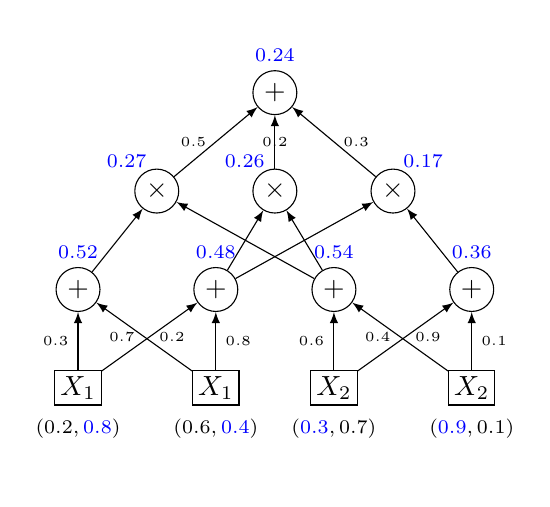
\begin{tikzpicture}
      \begin{scope}[every node/.style={circle,draw,inner sep=2pt}]
        \node[label={[label distance=-5pt]above:\scriptsize$\textcolor{blue}{0.24}$}] (root) at (0, 0) {$+$};
        \node[label={[label distance=-3pt]above left:\scriptsize$\textcolor{blue}{0.27}$}] (p1) at (-1.5, -1.25) {$\times$};
        \node[label={[label distance=-3pt]above left:\scriptsize$\textcolor{blue}{0.26}$}] (p2) at (0, -1.25) {$\times$};
        \node[label={[label distance=-3pt]above right:\scriptsize$\textcolor{blue}{0.17}$}] (p3) at (1.5, -1.25) {$\times$};
        \node[label={[label distance=-5pt]above:\scriptsize$\textcolor{blue}{0.52}$}] (s1) at (-2.5, -2.5) {$+$};
        \node[label={[label distance=-5pt]above:\scriptsize$\textcolor{blue}{0.48}$}] (s2) at (-0.75, -2.5) {$+$};
        \node[label={[label distance=-5pt]above:\scriptsize$\textcolor{blue}{0.54}$}] (s3) at (0.75, -2.5) {$+$};
        \node[label={[label distance=-5pt]above:\scriptsize$\textcolor{blue}{0.36}$}] (s4) at (2.5, -2.5) {$+$};
        \node[draw,fill=none,rectangle,label={[label distance=-10pt]below:\scriptsize$(0.2,
          \textcolor{blue}{0.8})$}] (x11) at (-2.5, -3.75) {${X}_1$};
        \node[draw,fill=none,rectangle,label={[label distance=-10pt]below:\scriptsize$(0.6,
          \textcolor{blue}{0.4})$}] (x12) at (-0.75, -3.75) {${X}_1$};
        \node[draw,fill=none,rectangle,label={[label
          distance=-10pt]below:\scriptsize$(\textcolor{blue}{0.3}, 0.7)$}] (x21) at (0.75, -3.75) {${X}_2$};
        \node[draw,fill=none,rectangle,label={[label
          distance=-10pt]below:\scriptsize$(\textcolor{blue}{0.9}, 0.1)$}] (x22) at (2.5, -3.75) {${X}_2$};
      \end{scope}
      \begin{scope}[every path/.style={->},>=latex]
        \draw (p1) -- node[left]{\tiny$0.5$} (root);
        \draw (p2) -- node{\tiny$0.2$} (root);
        \draw (p3) -- node[right]{\tiny$0.3$} (root);
        \draw (s1) -- (p1);
        \draw (s3) -- (p1);
        \draw (s2) -- (p2);
        \draw (s3) -- (p2);
        \draw (s2) -- (p3);
        \draw (s4) -- (p3);
        \draw (x11) -- node[left]{\tiny$0.3$} (s1);
        \draw (x12) -- node[left]{\tiny$0.7$} (s1);
        \draw (x11) -- node[right]{\tiny$0.2$} (s2);
        \draw (x12) -- node[right]{\tiny$0.8$} (s2);
        \draw (x21) -- node[left]{\tiny$0.6$} (s3);
        \draw (x22) -- node[left]{\tiny$0.4$} (s3);
        \draw (x21) -- node[right]{\tiny$0.9$} (s4);
        \draw (x22) -- node[right]{\tiny$0.1$} (s4);
      \end{scope}
    \end{tikzpicture}
  \end{center}
  \begin{equation*}
    P(\mathbf{e}=\{X_1=1,X_2=0\})=0.24
  \end{equation*}
\end{frame}

\begin{frame}
  \frametitle{Computing marginals}
  We compute marginals by summing out to $1$ missing variables' leaves. Let $\mathbf{X}=\{X_1=1\}$.
  We want to compute $P(\mathbf{X})$:
  \begin{center}
    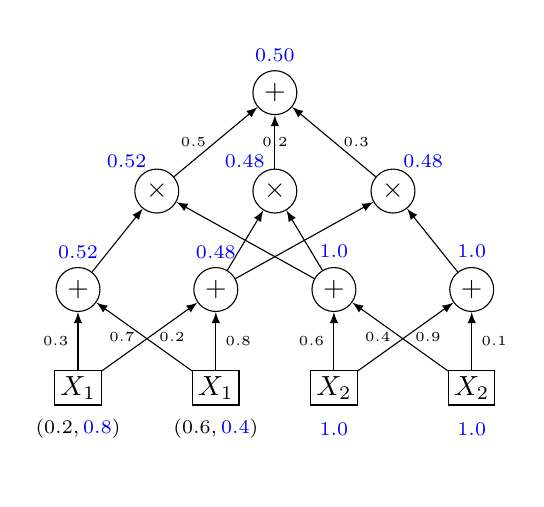
\begin{tikzpicture}
      \begin{scope}[every node/.style={circle,draw,inner sep=2pt}]
        \node[label={[label distance=-5pt]above:\scriptsize$\textcolor{blue}{0.50}$}] (root) at (0, 0) {$+$};
        \node[label={[label distance=-3pt]above left:\scriptsize$\textcolor{blue}{0.52}$}] (p1) at (-1.5, -1.25) {$\times$};
        \node[label={[label distance=-3pt]above left:\scriptsize$\textcolor{blue}{0.48}$}] (p2) at (0, -1.25) {$\times$};
        \node[label={[label distance=-3pt]above right:\scriptsize$\textcolor{blue}{0.48}$}] (p3) at (1.5, -1.25) {$\times$};
        \node[label={[label distance=-5pt]above:\scriptsize$\textcolor{blue}{0.52}$}] (s1) at (-2.5, -2.5) {$+$};
        \node[label={[label distance=-5pt]above:\scriptsize$\textcolor{blue}{0.48}$}] (s2) at (-0.75, -2.5) {$+$};
        \node[label={[label distance=-3pt]above:\scriptsize$\textcolor{blue}{1.0}$}] (s3) at (0.75, -2.5) {$+$};
        \node[label={[label distance=-3pt]above:\scriptsize$\textcolor{blue}{1.0}$}] (s4) at (2.5, -2.5) {$+$};
        \node[draw,fill=none,rectangle,label={[label distance=-10pt]below:\scriptsize$(0.2,
          \textcolor{blue}{0.8})$}] (x11) at (-2.5, -3.75) {${X}_1$};
        \node[draw,fill=none,rectangle,label={[label distance=-10pt]below:\scriptsize$(0.6,
          \textcolor{blue}{0.4})$}] (x12) at (-0.75, -3.75) {${X}_1$};
        \node[draw,fill=none,rectangle,label={[label
          distance=0pt]below:\scriptsize$\textcolor{blue}{1.0}$}] (x21) at (0.75, -3.75) {${X}_2$};
        \node[draw,fill=none,rectangle,label={[label
          distance=0pt]below:\scriptsize$\textcolor{blue}{1.0}$}] (x22) at (2.5, -3.75) {${X}_2$};
      \end{scope}
      \begin{scope}[every path/.style={->},>=latex]
        \draw (p1) -- node[left]{\tiny$0.5$} (root);
        \draw (p2) -- node{\tiny$0.2$} (root);
        \draw (p3) -- node[right]{\tiny$0.3$} (root);
        \draw (s1) -- (p1);
        \draw (s3) -- (p1);
        \draw (s2) -- (p2);
        \draw (s3) -- (p2);
        \draw (s2) -- (p3);
        \draw (s4) -- (p3);
        \draw (x11) -- node[left]{\tiny$0.3$} (s1);
        \draw (x12) -- node[left]{\tiny$0.7$} (s1);
        \draw (x11) -- node[right]{\tiny$0.2$} (s2);
        \draw (x12) -- node[right]{\tiny$0.8$} (s2);
        \draw (x21) -- node[left]{\tiny$0.6$} (s3);
        \draw (x22) -- node[left]{\tiny$0.4$} (s3);
        \draw (x21) -- node[right]{\tiny$0.9$} (s4);
        \draw (x22) -- node[right]{\tiny$0.1$} (s4);
      \end{scope}
    \end{tikzpicture}
  \end{center}
  \begin{equation*}
    P(\mathbf{X}=\{X_1=1\})=0.5
  \end{equation*}
\end{frame}

\begin{frame}
  \frametitle{The task}

  Given a track, bot must autonomously complete the whole course without going off road. The only
  available input is a single frontal camera.

  \begin{figure}[h]
    \centering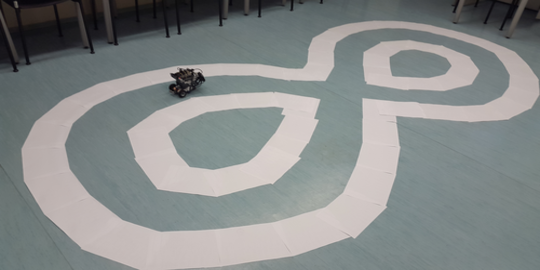
\includegraphics[width=0.475\textwidth]{imgs/track_1_resize.png}
    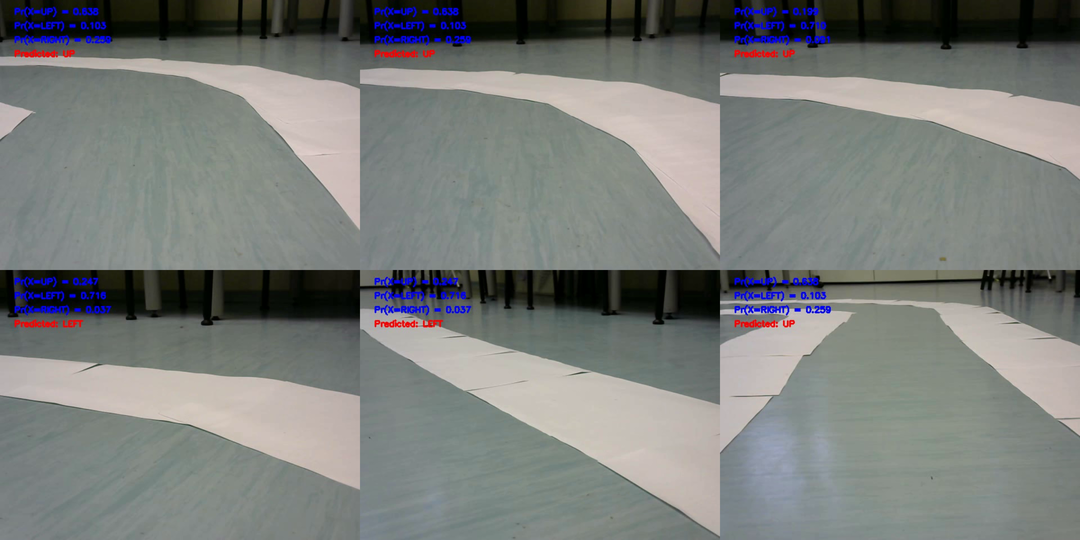
\includegraphics[width=0.475\textwidth]{imgs/demo_merged_pairs_small.png}
  \end{figure}

  Decision making must be done in real-time under a resource constrained, low-budget robot
  environment.

\end{frame}

\begin{frame}
  \frametitle{Why SPNs?}

  \begin{itemize}
    \item Probabilistic semantics (efficiently compute probability of input and detect outliers);
    \item Easy to build and debug (efficient algorithms for learning structure from data;
      probabilistic semantics);
    \item No need for heavy packages (e.g. Tensorflow);
    \item Good performance with much smaller models;
    \item Not been tried ``in the wild'' yet.
  \end{itemize}
\end{frame}

\begin{frame}
  \frametitle{Robot}

  \begin{multicols}{2}
    \textbf{Raspberry Pi 3 Model B}
    \begin{description}
      \item[CPU:] Quad Core 1.2GHz Broadcom BCM2837 64bit ARMv7
      \item[Memory:] 1GB RAM
      \item[Storage:] 16GB SSD
    \end{description}
    \textbf{Lego Mindstorms NXT}
    \begin{description}
      \item[CPU:] Atmel AT91SAM7S256 48MHz 32bit ARMv4
      \item[Memory:] 64KB RAM
      \item[Storage:] 256KB Flash
    \end{description}
  \end{multicols}

  \begin{figure}
    \centering
    \begin{minipage}{0.3\textwidth}
      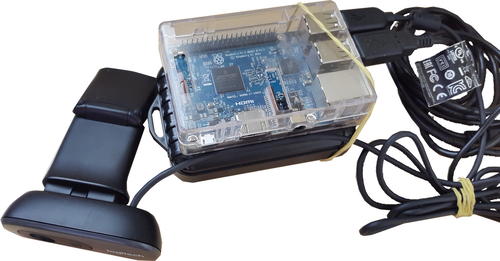
\includegraphics[width=\linewidth]{imgs/berry.png}
    \end{minipage}
    $+$
    \begin{minipage}{0.3\textwidth}
      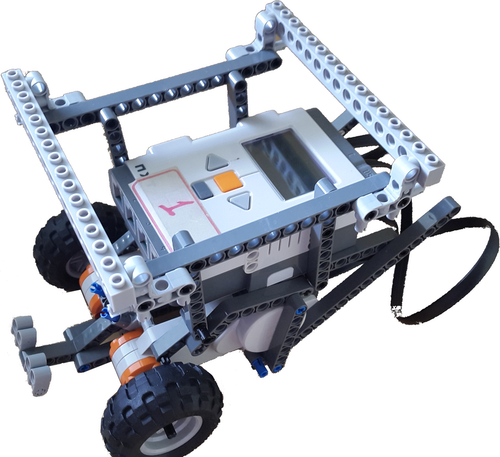
\includegraphics[width=\linewidth]{imgs/brick.png}
    \end{minipage}
    $=$
    \begin{minipage}{0.3\textwidth}
      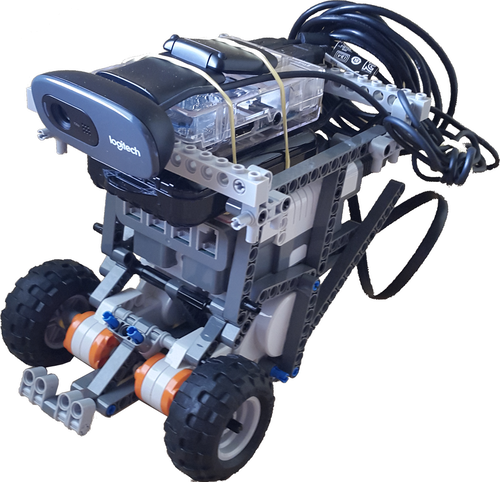
\includegraphics[width=\linewidth]{imgs/robot.png}
    \end{minipage}
  \end{figure}
\end{frame}

\begin{frame}
  \frametitle{Modelling}

  Every pixel $X_i$ is a variable in the distribution represented by the SPN, i.e. no additional
  feature extraction, end-to-end.

  Two architectures:
  \begin{description}
    \item[GD:] LearnSPN with $k$-means and $G$-test
    \item[DV:] Clustering on Variables
  \end{description}
  Three weight setups:
  \begin{description}
    \item[g:] Generative gradient descent
    \item[d:] Discriminative gradient descent
    \item[s:] Proportional weights for GD, random weights for DV
  \end{description}
\end{frame}

\begin{frame}
  \frametitle{Experiments}

  \textbf{Training}
  \begin{itemize}
    \item Trained models with samples from a single simple track;
    \item 500 training samples (corresponding to 0.9\% of the dataset);
    \item Training took from 30 mins to 9 hours (time dependent on parameters, pre-processing and
      learning algorithms) on an Intel i7-4500U 1.8GHz CPU.
  \end{itemize}

  \textbf{Evaluation}
  \begin{itemize}
    \item Tests run on three different tracks;
    \item Different floor and lighting conditions from training dataset.
  \end{itemize}

  \begin{figure}
    \centering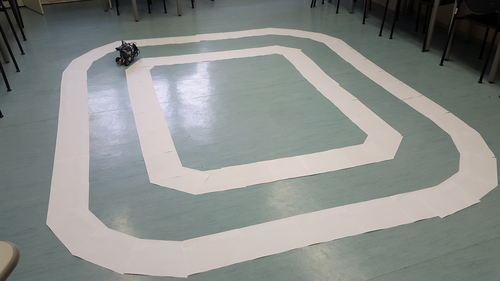
\includegraphics[width=0.3\textwidth]{imgs/track_0.png}
    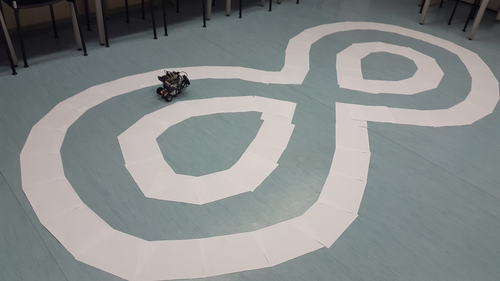
\includegraphics[width=0.3\textwidth]{imgs/track_1.png}
    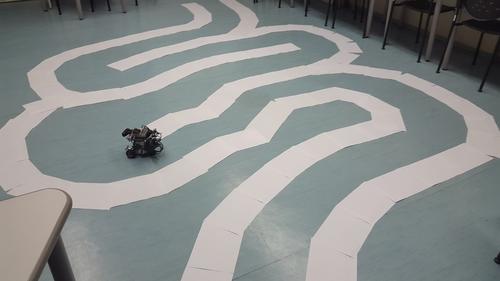
\includegraphics[width=0.3\textwidth]{imgs/track_2.png}
  \end{figure}
\end{frame}

\begin{frame}
  \frametitle{Dataset}

  Dataset used: \cite{moraes18}

  \begin{figure}
    \centering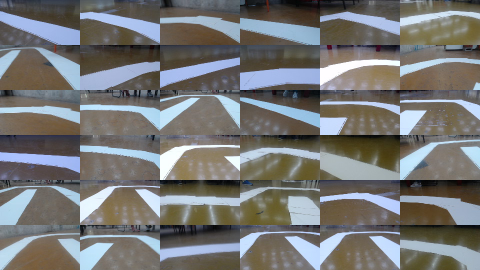
\includegraphics[height=0.5\textheight]{imgs/montage_raw.png}
  \end{figure}

  Lane tracking dataset with $80\times 45$ RGB images. Each labeled with either UP, LEFT or RIGHT.
\end{frame}

\begin{frame}
  \frametitle{Self-driving as image classification}

  \begin{figure}
    \begin{subfigure}{0.3\linewidth}
      \centering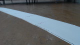
\includegraphics{imgs/sample_left.png}
      \captionsetup{justification=centering}
      \caption*{LEFT}
    \end{subfigure}
    \begin{subfigure}{0.3\linewidth}
      \centering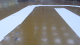
\includegraphics{imgs/sample_up.png}
      \captionsetup{justification=centering}
      \caption*{UP}
    \end{subfigure}
    \begin{subfigure}{0.3\linewidth}
      \centering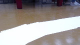
\includegraphics{imgs/sample_right.png}
      \captionsetup{justification=centering}
      \caption*{RIGHT}
    \end{subfigure}
  \end{figure}

  \begin{figure}
    \centering\includegraphics[height=0.35\textheight]{imgs/train_track.png}
  \end{figure}

  \begin{center}
    Training track in \cite{moraes18}.
  \end{center}
\end{frame}

\begin{frame}
  \frametitle{Training}

  Training was done on an Intel i7-4500U CPU \@ 1.80 Hz.

  \begin{figure}[h]
    \centering
    \resizebox{\columnwidth}{!}{
      \begin{tikzpicture}
        \node[inner sep=0pt, label=Raw] (raw) at (0, 0)
          {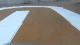
\includegraphics{imgs/pipe_raw.png}};
        \node[inner sep = 0pt, right = 2.0cm of raw, label=Gray] (gray)
          {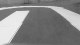
\includegraphics{imgs/pipe_gray.png}};
        \node[inner sep = 0pt, right = 2.0cm of gray, label=Binarized] (bin)
          {
\includegraphics{imgs/pipe_bin.png}};
        \node[rectangle, rounded corners, draw, below = 2.0cm of gray,
          minimum size=2cm] (weights) {LearnWeight};
        \node[rectangle, rounded corners, draw, right = 2.0cm of weights,
          minimum size=2cm] (struct) {LearnStructure};
        \node[cylinder, shape border rotate=90, draw, left = 2.0cm of weights,
          label=below:SaveDisk, minimum width=2cm, minimum height=1cm] (save) {};
        \node[inner sep = 0.75cm, rectangle, dashed, draw, thick, fit=(raw) (gray) (bin),
          label=above:\textbf{Pre-processing}] (pp) {};
        \node[inner sep = 0.5cm, rectangle, dotted, draw, thick, fit=(struct) (weights) (save),
          label=above:\textbf{Training}] (train) {};
        \draw[->,thick] (raw.east) -- (gray.west);
        \draw[->,thick] (gray.east) -- (bin.west);
        \draw[->,thick] let \p1 = (train.east), \p2 = (pp.east) in
          (\p2) -- ($ (\p2) + (0.5, 0) $) -- ($ (\x2, \y1) + (0.5, 0) $) -- (\p1);
        \draw[->,thick] (struct.west) -- (weights.east);
        \draw[->,thick] (weights.west) -- (save.east);
      \end{tikzpicture}
    }
  \end{figure}

  Saved SPN was then passed to the Raspberry.
\end{frame}

\begin{frame}
  \frametitle{Prediction}

  \begin{figure}[h]
    \centering
    \resizebox{\columnwidth}{!}{
      \begin{tikzpicture}
        \node[inner sep=0pt, label=Raw] (raw) at (0, 0)
          {
\includegraphics{imgs/pipe_out_raw.png}};
        \node[inner sep = 0pt, right = 2.0cm of raw, label=Gray] (gray)
          {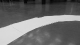
\includegraphics{imgs/pipe_out_gray.png}};
        \node[inner sep = 0pt, right = 2.0cm of gray, label=Binarized] (bin)
          {
\includegraphics{imgs/pipe_out_bin.png}};
        \node[inner sep = 0.75cm, rectangle, dashed, draw, thick, fit=(raw) (gray) (bin),
          label=above:\textbf{Pre-processing}] (pp) {};
        \node[cylinder, shape border rotate=90, draw, below = 2.0cm of raw,
          label=below:LoadDisk, minimum width=2cm, minimum height = 1cm] (load) {};
        \node[rectangle, rounded corners, draw, right = 2.0cm of load,
          minimum size=2cm] (build) {BuildSPN};
        \node[rectangle, rounded corners, draw, right = 2.0cm of build, right = 3.0cm of build,
          minimum size=2cm] (infer) {Inference};
        \node[inner sep = 0.5cm, rectangle, dotted, draw, thick, fit=(load) (build),
          label=below:\textbf{SPN loading}] (create) {};
        \node[below = 1.0cm of infer] (pred) {Predicted: RIGHT};
        \draw[->,thick] (raw.east) -- (gray.west);
        \draw[->,thick] (gray.east) -- (bin.west);
        \draw[->,thick] let \p1 = (infer.east), \p2 = (pp.east) in
          (\p2) -- ($ (\p2) + (0.5, 0) $) -- ($ (\x2, \y1) + (0.5, 0) $) -- (\p1);
        \draw[->,thick] (load) -- (build);
        \draw[->,thick] (create) -- (infer);
        \draw[->,thick] (infer) -- (pred);
      \end{tikzpicture}
    }
  \end{figure}
\end{frame}

\begin{frame}
  \frametitle{Chosen models}

  \begin{description}
    \item[Model 1:] $Q_4$, \textbf{GD+d}
      \begin{description}
        \item[Accuracy:] 78.2\%
        \item[Desktop time:] 170ms
        \item[Berry time:] 700ms
      \end{description}
    \item[Model 2:] $Q_6$, \textbf{GD+d}
      \begin{description}
        \item[Accuracy:] 74.4\%
        \item[Desktop time:] 50ms
        \item[Berry time:] 150ms
      \end{description}
    \item[Model 3:] $\emptyset$, \textbf{GD+d}
      \begin{description}
        \item[Accuracy:] 62.4\%
        \item[Desktop time:] $<$ 10ms
        \item[Berry time:] 75ms
      \end{description}
  \end{description}
\end{frame}

\begin{frame}
  \frametitle{Comparison to neural networks}

  Comparison to~\cite{moraes18}:

  \begin{table}
    \centering
    \begin{tabular}{l|c|c}
      \textbf{Model} & \textbf{Accuracy (\%)} & \textbf{Speed (seconds)}\\
      \hline
      DFN & 81.3 & $\approx$1.35\\
      CNN & 80.6 & $\approx$1.35\\
      \hline
      $Q_4$, GD-SPN+d & 78.2 & $\approx$0.70\\
      $Q_6$, GD-SPN+d & 74.4 & $\approx$0.15\\
      GD-SPN+d & 62.4 & $\approx$0.07
    \end{tabular}
  \end{table}

  Neural networks were slightly more accurate, but real-time prediction with them is
  unfeasible.\\~\\

  Our implementation did not make use of the GPU, which could increase speed dramatically.\\~\\

  Real-time decision making poses new challenges: timely decisions are often more important than
  accurate decisions.

\end{frame}

\begin{frame}
  \frametitle{``Real world'' scenario}

  \footnotesize\centering\textbf{\href{https://youtu.be/vhpWQDX2cQU}{Mobile Robot Self-Driving Through Image Classification Using
  Discriminative Learning of Sum-Product Networks --- YouTube}}
  (\url{https://youtu.be/vhpWQDX2cQU})
\end{frame}

\begin{frame}
  \frametitle{Implementation}
  \centering
  \large\textbf{Inference and learning:} \href{https://github.com/RenatoGeh/gospn}{GoSPN}
  (\url{https://github.com/RenatoGeh/gospn})\\~\\

  \textbf{Mobile robot implementation:} \href{https://github.com/RenatoGeh/godrive}{GoDrive}
  (\url{https://github.com/RenatoGeh/godrive})

\end{frame}

\begin{frame}
  \begin{center}
    \textbf{Thank you.\\~\\Questions?}
  \end{center}
\end{frame}

\begin{frame}
  \frametitle{Sum-product networks}

  \begin{definition}[Sum-product network]~\\
    A sum-product network (SPN) is a DAG where each node $n$ is either:
    \begin{enumerate}
      \item A tractable univariate probability distribution;
      \item A product of SPNs: $v_n=\prod_{j\in\Ch(n)}v_j$; or
      \item A weighted sum of SPNs: $v_n=\sum_{j\in\Ch(n)}w_{n,j}v_j$.
    \end{enumerate}
    Where $v_n$ is the value of node $n$, $\Ch(n)$ its set of children and $w_{n,j}$ the weight of
    edge $n\to j$.
  \end{definition}
\end{frame}

\begin{frame}
  \frametitle{Accuracy}
  \footnotesize
  \begin{table}[h]
    \centering
    \begin{tabular}{l|c|c|c|c|c|c}
      \hline
      \multicolumn{1}{c}{\bfseries Accuracy (\%)} & \multicolumn{1}{c}{\bfseries DV+g} &
      \multicolumn{1}{c}{\bfseries DV+d} & \multicolumn{1}{c}{\bfseries DV+s} &
      \multicolumn{1}{c}{\bfseries GD+g} & \multicolumn{1}{c}{\bfseries GD+d} &
      \multicolumn{1}{c}{\bfseries GD+s}\\
      \hline
      $B$         & 78.8 & 78.8 & 78.8 & 82.8 & 83.8 & 85.0\\
      $Q_2$       & 78.6 & 78.0 & 78.0 & 78.6 & 80.4 & 79.4\\
      $Q_2+E$     & 76.6 & 76.6 & 76.8 & 79.6 & 82.8 & 81.8\\
      $Q_3$       & 77.4 & 77.4 & 77.4 & 77.6 & 80.2 & 79.8\\
      $Q_3+E$     & 70.4 & 76.6 & 76.6 & 79.2 & 81.2 & 77.4\\
      $Q_4$       & 78.2 & 78.4 & 78.2 & 76.0 & \textbf{78.2} & 76.4\\
      $Q_4+E$     & 76.6 & 76.6 & 76.8 & 76.0 & 74.6 & 80.6\\
      $Q_5$       & 77.8 & 78.4 & 78.4 & 77.6 & 74.0 & 73.8\\
      $Q_5+E$     & 76.6 & 76.6 & 76.6 & 72.0 & 72.8 & 72.0\\
      $Q_6$       & 77.4 & 78.4 & 78.4 & 75.2 & \textbf{74.4} & 72.0\\
      $Q_6+E$     & 76.0 & 76.4 & 76.4 & 73.0 & 75.0 & 73.6\\
      $Q_7$       & 78.2 & 78.4 & 78.4 & 62.8 & 72.2 & 71.4\\
      $Q_7+E$     & 76.2 & 76.4 & 76.4 & 70.6 & 71.4 & 71.6\\
      $\emptyset$ & 78.0 & 78.4 & 78.4 & 62.4 & \textbf{62.4} & 62.4\\
      $E$         & 76.4 & 76.4 & 76.4 & 60.4 & 60.0 & 61.2\\
    \end{tabular}
  \end{table}

  \begin{center}
    $B$: binarization, $Q_n$: $n$-bit quantization, $E$: histogram equalization.
  \end{center}
\end{frame}

\begin{frame}
  \frametitle{Inference time}
  \footnotesize
  \begin{table}[h]
    \centering
    \begin{tabular}{l|c|c|c|c|c|c}
      \hline
      \multicolumn{1}{c}{\bfseries Inference (secs)} & \multicolumn{1}{c}{\bfseries DV+g} &
      \multicolumn{1}{c}{\bfseries DV+d} & \multicolumn{1}{c}{\bfseries DV+s} &
      \multicolumn{1}{c}{\bfseries GD+g} & \multicolumn{1}{c}{\bfseries GD+d} &
      \multicolumn{1}{c}{\bfseries GD+s}\\
      \hline
      $B$         & 0.23 & 0.25 & 0.25 & 0.38 & 0.37 & 0.31 \\
      $Q_2$       & 0.22 & 0.24 & 0.23 & 0.28 & 0.34 & 0.16 \\
      $Q_2+E$     & 0.22 & 0.23 & 0.23 & 0.38 & 0.30 & 0.27 \\
      $Q_3$       & 0.22 & 0.23 & 0.22 & 0.22 & 0.32 & 0.17 \\
      $Q_3+E$     & 0.22 & 0.23 & 0.22 & 0.34 & 0.32 & 0.31 \\
      $Q_4$       & 0.22 & 0.22 & 0.23 & 0.16 & \textbf{0.17} & 0.13 \\
      $Q_4+E$     & 0.23 & 0.27 & 0.29 & 0.13 & 0.14 & 0.13 \\
      $Q_5$       & 0.22 & 0.26 & 0.28 & 0.07 & 0.05 & 0.02 \\
      $Q_5+E$     & 0.22 & 0.29 & 0.25 & 0.05 & 0.05 & 0.02 \\
      $Q_6$       & 0.23 & 0.24 & 0.23 & 0.04 & \textbf{0.05} & 0.01 \\
      $Q_6+E$     & 0.22 & 0.24 & 0.28 & 0.03 & 0.04 & 0.02 \\
      $Q_7$       & 0.23 & 0.23 & 0.26 & 0.03 & 0.01 & 0.01 \\
      $Q_7+E$     & 0.22 & 0.26 & 0.24 & 0.01 & 0.01 & 0.01 \\
      $\emptyset$ & 0.22 & 0.26 & 0.23 & 0.02 & \textbf{0.01} & 0.01 \\
      $E$         & 0.23 & 0.23 & 0.22 & 0.01 & 0.01 & 0.02 \\
    \end{tabular}
  \end{table}

  \begin{center}
    $B$: binarization, $Q_n$: $n$-bit quantization, $E$: histogram equalization.
  \end{center}
\end{frame}

\begin{frame}[t,allowframebreaks]
  \frametitle{References}
  \printbibliography[heading=none]
  \nocite{*}
\end{frame}

\end{document}
